\section{About}

\begin{wrapfigure}{R}{0.3\textwidth}
\centering
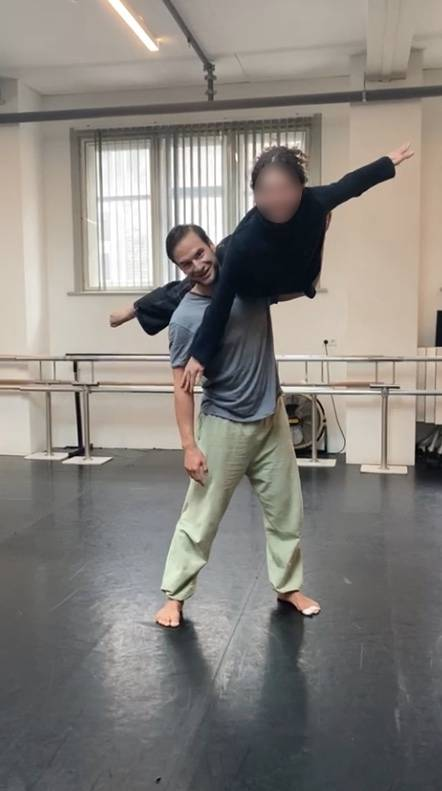
\includegraphics[width=0.25\textwidth]{images/about.jpg}
\end{wrapfigure}

This little book is written by me for taking my personal notes in a digital form, so it also might be used by others, by beginners and non-beginners alike, who are interested in getting more acquainted with the theoretical background of the fine art of Contact Improvisation Dance, or simply \textbf{CI} for short as of now (sometimes also called \textit{contact} in the community).

Whatever is written here does not claim to hold any absolute, objective truth, but merely is a manifestation of my own personal, subjective collection of thoughts and opinions. Additionally to that, I summarized all the information I stumbled upon along my path of exploration, might it be oral teachings, direct or indirect, or written information found in books and on the internet. I am also trying to rely on a more "innocent" approach and write about my own experiences and interpretation of whatever seems to be true to me, which is of course very much colored by me as a person and my personal (movement) background.

Speaking of my background: It is mainly Japanese (Karate, Aikido) and Chinese Martial Arts (Taijiquan), and as such, my focus lies more on a practical approach, where "form follows function", and less about any aesthetic aspects as many might consider be an essential part of dancing in a more narrow definition. Furthermore, as a bodyworker (Shiatsu Therapy and Neo-Tantrism), I emphasize the importance of the non-verbal communication (Non-Violent Communication) aspect of movement and touch. Whether we express ourselves in a free form art or the way we interact with others without words.

For me personally, the looks are irrelevant, and "right" is what is pragmatic, meaning efficient in time and space (thinking of anatomy, physics, and biomechanics), and as well whatever is in alignment with the principles of CI. Besides those more physical aspects, the psychological aspect should be granted at least half of the attention: The benefit for one's mental health, the ability to get to know oneself and others more deeply, and of course a more philosophical/spiritual path which can also be walked with the help of this deep art.
